%\documentclass[landscape,a0b,final,a4resizeable]{a0poster}
\documentclass[landscape,a0b,final]{a0poster}
%\documentclass[portrait,a0b,final,a4resizeable]{a0poster}
%\documentclass[portrait,a0b,final]{a0poster}
%%% Option "a4resizeable" makes it possible ot resize the
%   poster by the command: psresize -pa4 poster.ps poster-a4.ps
%   For final printing, please remove option "a4resizeable" !!

\usepackage{epsfig}
\usepackage{multicol}
\usepackage{pstricks,pst-grad}



%%%%%%%%%%%%%%%%%%%%%%%%%%%%%%%%%%%%%%%%%%%
% Definition of some variables and colors
%\renewcommand{\rho}{\varrho}
%\renewcommand{\phi}{\varphi}
\setlength{\columnsep}{3cm}
\setlength{\columnseprule}{2mm}
\setlength{\parindent}{0.0cm}



%%%%%%%%%%%%%%%%%%%%%%%%%%%%%%%%%%%%%%%%%%%%%%%%%%%%
%%%               Background                     %%%
%%%%%%%%%%%%%%%%%%%%%%%%%%%%%%%%%%%%%%%%%%%%%%%%%%%%

\newcommand{\background}[3]{
  \newrgbcolor{cgradbegin}{#1}
  \newrgbcolor{cgradend}{#2}
  \psframe[fillstyle=gradient,gradend=cgradend,
  gradbegin=cgradbegin,gradmidpoint=#3](0.,0.)(1.\textwidth,-1.\textheight)
}



%%%%%%%%%%%%%%%%%%%%%%%%%%%%%%%%%%%%%%%%%%%%%%%%%%%%
%%%                Poster                        %%%
%%%%%%%%%%%%%%%%%%%%%%%%%%%%%%%%%%%%%%%%%%%%%%%%%%%%

\newenvironment{poster}{
  \begin{center}
  \begin{minipage}[c]{0.98\textwidth}
}{
  \end{minipage} 
  \end{center}
}



%%%%%%%%%%%%%%%%%%%%%%%%%%%%%%%%%%%%%%%%%%%%%%%%%%%%
%%%                pcolumn                       %%%
%%%%%%%%%%%%%%%%%%%%%%%%%%%%%%%%%%%%%%%%%%%%%%%%%%%%

\newenvironment{pcolumn}[1]{
  \begin{minipage}{#1\textwidth}
  \begin{center}
}{
  \end{center}
  \end{minipage}
}



%%%%%%%%%%%%%%%%%%%%%%%%%%%%%%%%%%%%%%%%%%%%%%%%%%%%
%%%                pbox                          %%%
%%%%%%%%%%%%%%%%%%%%%%%%%%%%%%%%%%%%%%%%%%%%%%%%%%%%

\newrgbcolor{lcolor}{0. 0. 0.80}
\newrgbcolor{gcolor1}{1. 1. 1.}
\newrgbcolor{gcolor2}{.80 .80 1.}

\newcommand{\pbox}[4]{
\psshadowbox[#3]{
\begin{minipage}[t][#2][t]{#1}
#4
\end{minipage}
}}



%%%%%%%%%%%%%%%%%%%%%%%%%%%%%%%%%%%%%%%%%%%%%%%%%%%%
%%%                myfig                         %%%
%%%%%%%%%%%%%%%%%%%%%%%%%%%%%%%%%%%%%%%%%%%%%%%%%%%%
% \myfig - replacement for \figure
% necessary, since in multicol-environment 
% \figure won't work

\newcommand{\myfig}[3][0]{
\begin{center}
  \vspace{1.5cm}
  \includegraphics[width=#3\hsize,angle=#1]{#2}
  \nobreak\medskip
\end{center}}



%%%%%%%%%%%%%%%%%%%%%%%%%%%%%%%%%%%%%%%%%%%%%%%%%%%%
%%%                mycaption                     %%%
%%%%%%%%%%%%%%%%%%%%%%%%%%%%%%%%%%%%%%%%%%%%%%%%%%%%
% \mycaption - replacement for \caption
% necessary, since in multicol-environment \figure and
% therefore \caption won't work

%\newcounter{figure}
\setcounter{figure}{1}
\newcommand{\mycaption}[1]{
  \vspace{0.5cm}
  \begin{quote}
    {{\sc Figure} \arabic{figure}: #1}
  \end{quote}
  \vspace{1cm}
  \stepcounter{figure}
}



%%%%%%%%%%%%%%%%%%%%%%%%%%%%%%%%%%%%%%%%%%%%%%%%%%%%%%%%%%%%%%%%%%%%%%
%%% Begin of Document
%%%%%%%%%%%%%%%%%%%%%%%%%%%%%%%%%%%%%%%%%%%%%%%%%%%%%%%%%%%%%%%%%%%%%%

\begin{document}

\background{1. 1. 1.}{1. 1. 1.}{0.5}

\vspace*{2cm}


\newrgbcolor{lightblue}{0. 0. 0.80}
\newrgbcolor{white}{1. 1. 1.}
\newrgbcolor{whiteblue}{.80 .80 1.}


\begin{poster}

%%%%%%%%%%%%%%%%%%%%%
%%% Header
%%%%%%%%%%%%%%%%%%%%%
\begin{center}
\begin{pcolumn}{0.98}

\pbox{0.95\textwidth}{}{linewidth=2mm,framearc=0.3,linecolor=lightblue,fillstyle=gradient,gradangle=0,gradbegin=white,gradend=whiteblue,gradmidpoint=1.0,framesep=1em}{

%%% Unisiegel
\begin{minipage}[c][9cm][c]{0.1\textwidth}
  \begin{center}
    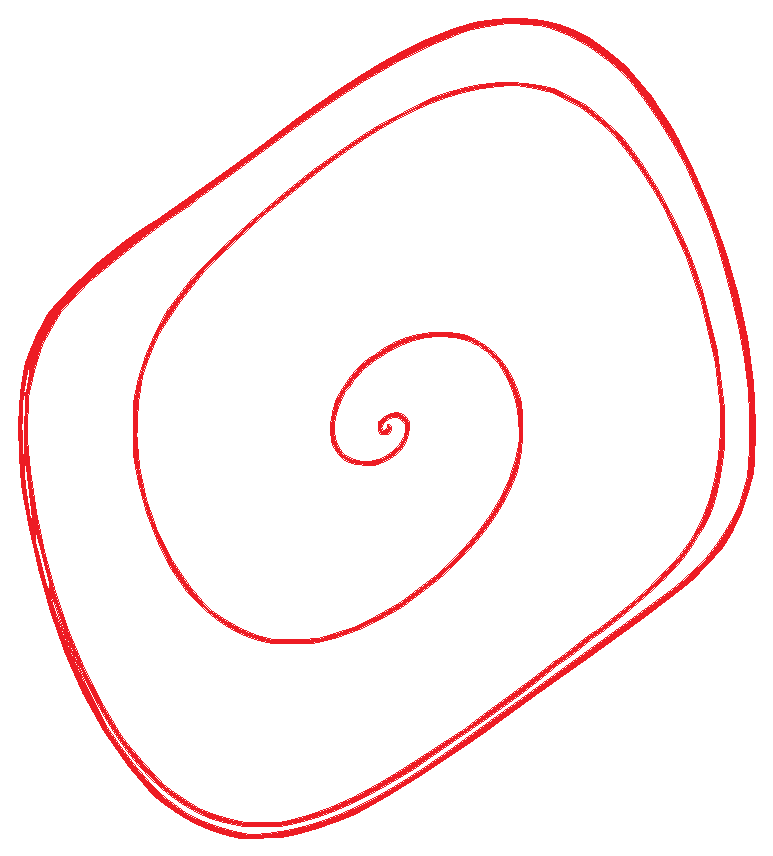
\includegraphics[width=7cm,angle=0]{gklogo.eps}
  \end{center}
\end{minipage}
%%% Titel
\begin{minipage}[c][9cm][c]{0.78\textwidth}
  \begin{center}
    {\sc \Huge This is the Title of your Poster}\\[10mm]
    {\Large A. Author1, B. Author2 and C. Author3\\[7.5mm]
    Institute of Poster--Design, University, Your City, Country}
  \end{center}
\end{minipage}
%%% GK-Logo
\begin{minipage}[c][9cm][c]{0.1\textwidth}
  \begin{center}
    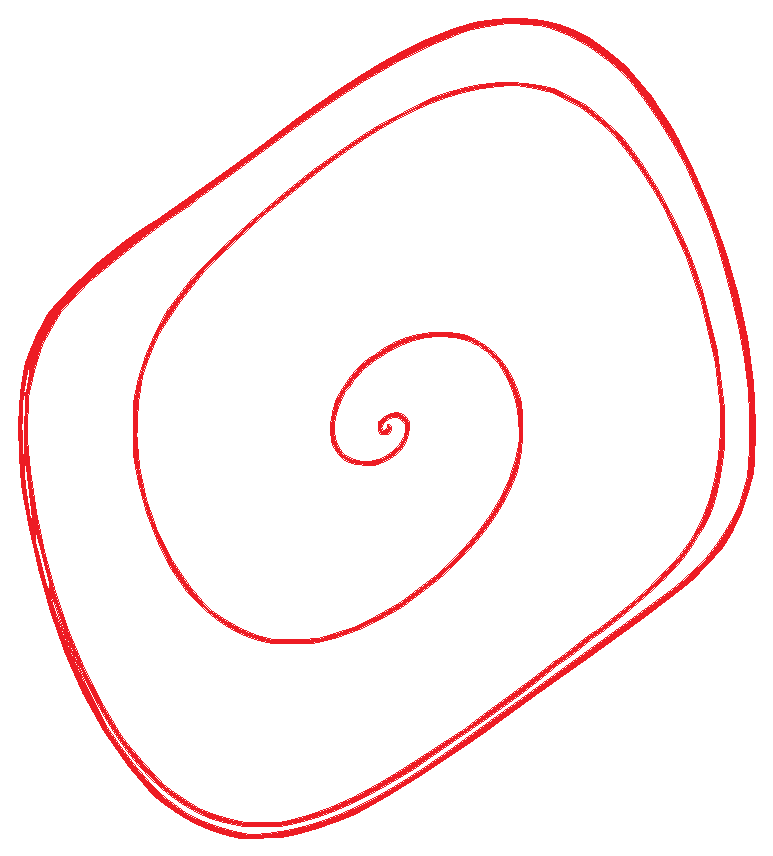
\includegraphics[width=7cm,angle=0]{gklogo.eps}
  \end{center}
\end{minipage}

}
\end{pcolumn}
\end{center}


\vspace*{2cm}



%%%%%%%%%%%%%%%%%%%%%
%%% Content
%%%%%%%%%%%%%%%%%%%%%
\begin{center}
\begin{pcolumn}{0.32}
\pbox{0.9\textwidth}{30cm}{linewidth=2mm,framearc=0.1,linecolor=lightblue,fillstyle=gradient,gradangle=0,gradbegin=white,gradend=white,gradmidpoint=1.0,framesep=1em}{

%%% Abstract
\begin{center}\pbox{0.8\textwidth}{}{linewidth=2mm,framearc=0.1,linecolor=lightblue,fillstyle=gradient,gradangle=0,gradbegin=white,gradend=whiteblue,gradmidpoint=1.0,framesep=1em}{\begin{center}Abstract\end{center}}\end{center}
\vspace{1.25cm}

This is your abstract of this poster or just put your abstract of your
paper here... This is your abstract of this poster or just put your
abstract of your paper here... This is your abstract of this poster or
just put your abstract of your paper here... This is your abstract of
this poster or just put your abstract of your paper here... This is
your abstract of this poster or just put your abstract of your paper
here... This is your abstract of this poster or just put your abstract
of your paper here... This is your abstract of this poster or just put
your abstract of your paper here...



%%% Introduction
\vspace{2cm}\begin{center}\pbox{0.8\textwidth}{}{linewidth=2mm,framearc=0.1,linecolor=lightblue,fillstyle=gradient,gradangle=0,gradbegin=white,gradend=whiteblue,gradmidpoint=1.0,framesep=1em}{\begin{center}Introduction\end{center}}\end{center}\vspace{1.25cm}

Your text with scientific results or what ever... Your text with
scientific results or what ever... Your text with scientific results or
what ever... Your text with scientific results or what ever... Your
text with scientific results or what ever... Your text with scientific
results or what ever... Your text with scientific results or what
ever... Your text with scientific results or what ever... Your text
with scientific results or what ever...

Your text with scientific results or what ever... Your text with
scientific results or what ever... Your text with scientific results or
what ever... Your text with scientific results or what ever... Your
text with scientific results or what ever... Your text with scientific
results or what ever... Your text with scientific results or what
ever...
}
\end{pcolumn}
\begin{pcolumn}{0.32}
\pbox{0.9\textwidth}{30cm}{linewidth=2mm,framearc=0.1,linecolor=lightblue,fillstyle=gradient,gradangle=0,gradbegin=white,gradend=white,gradmidpoint=1.0,framesep=1em}{

Your text with scientific results or what ever... Your text with
scientific results or what ever... Your text with scientific results or
what ever... Your text with scientific results or what ever... Your
text with scientific results or what ever...

\begin{equation}\label{eqn:first}
  \sum_{i=1}^{N} x = \frac{(N+1)N}{2}
\end{equation}

Your text with scientific results or what ever...
equation~\ref{eqn:first}... Your text with scientific results or what
ever... Your text with scientific results or what ever... Your text
with scientific results or what ever... Your text with scientific
results or what ever... Your text with scientific results or what
ever... Your text with scientific results or what ever... Your text
with scientific results or what ever... Your text with scientific
results or what ever... Your text with scientific results or what
ever...

%%% Section
\vspace{2cm}\begin{center}\pbox{0.8\textwidth}{}{linewidth=2mm,framearc=0.1,linecolor=lightblue,fillstyle=gradient,gradangle=0,gradbegin=white,gradend=whiteblue,gradmidpoint=1.0,framesep=1em}{\begin{center}Section\end{center}}\end{center}\vspace{1.25cm}

\cite{Aut2001} Your
text with scientific results or what ever... Your text with scientific
results or what ever... Your text with scientific results or what
ever... Your text with scientific results or what ever... Your text
with scientific results or what ever... Your text with scientific
results or what ever... Your text with scientific results or what
ever... Your text with scientific results or what ever... Your text
with scientific results or what ever... Your text with scientific
results or what ever...

}
\end{pcolumn}
\begin{pcolumn}{0.32}
\pbox{0.9\textwidth}{30cm}{linewidth=2mm,framearc=0.1,linecolor=lightblue,fillstyle=gradient,gradangle=0,gradbegin=white,gradend=white,gradmidpoint=1.0,framesep=1em}{

Your text with scientific results or what ever... Your text with
scientific results or what ever... Your text with scientific results or
what ever... Your text with scientific results or what ever... Your
text with scientific results or what ever... Your text with scientific
results or what ever... Your text with scientific results or what
ever... Your text with scientific results or what ever... Your text
with scientific results or what ever...

%%% Figures:
\begin{center}
  % first argument: eps-file
  % second argument: stretching-factor relative to Column-width (<1)
  % optional argument: rotation angle (0-360), default=0
  \myfig[30]{gklogo.eps}{0.15}
  \mycaption{Emblem of the University of Regensburg (rotated by $30^\circ$). Emblem of the University of Regensburg (rotated by $30^\circ$).}
\end{center}

Your text with scientific results or what ever... Your text with
scientific results or what ever... Your text with scientific results or
what ever... Your text with scientific results or what ever... Your
text with scientific results or what ever... Your text with scientific
results or what ever... Your text with scientific results or what
ever... Your text with scientific results or what ever... Your text
with scientific results or what ever...

%%% References
\bibliographystyle{alpha}
\bibliography{poster.bib}


}
\end{pcolumn}
\end{center}



\vspace*{2cm}

%%% Begin of Multicols-Enviroment
\begin{multicols}{3}


%%% Abstract
\begin{center}\pbox{0.8\columnwidth}{}{linewidth=2mm,framearc=0.1,linecolor=lightblue,fillstyle=gradient,gradangle=0,gradbegin=white,gradend=whiteblue,gradmidpoint=1.0,framesep=1em}{\begin{center}Abstract\end{center}}\end{center}
\vspace{1.25cm}

This is your abstract of this poster or just put your abstract of your
paper here... This is your abstract of this poster or just put your
abstract of your paper here... This is your abstract of this poster or
just put your abstract of your paper here... This is your abstract of
this poster or just put your abstract of your paper here... This is
your abstract of this poster or just put your abstract of your paper
here... This is your abstract of this poster or just put your abstract
of your paper here... This is your abstract of this poster or just put
your abstract of your paper here...


%%% Introduction
\vspace{2cm}\begin{center}\pbox{0.8\columnwidth}{}{linewidth=2mm,framearc=0.1,linecolor=lightblue,fillstyle=gradient,gradangle=0,gradbegin=white,gradend=whiteblue,gradmidpoint=1.0,framesep=1em}{\begin{center}Introduction\end{center}}\end{center}\vspace{1.25cm}

Your text with scientific results or what ever... Your text with
scientific results or what ever... Your text with scientific results or
what ever... Your text with scientific results or what ever... Your
text with scientific results or what ever... Your text with scientific
results or what ever... Your text with scientific results or what
ever... Your text with scientific results or what ever... Your text
with scientific results or what ever...

Your text with scientific results or what ever... Your text with
scientific results or what ever... Your text with scientific results or
what ever... Your text with scientific results or what ever... Your
text with scientific results or what ever... Your text with scientific
results or what ever... Your text with scientific results or what
ever...

\begin{equation}\label{eqn:first}
  \sum_{i=1}^{N} x = \frac{(N+1)N}{2}
\end{equation}

Your text with scientific results or what ever...
equation~\ref{eqn:first}... Your text with scientific results or what
ever... Your text with scientific results or what ever... Your text
with scientific results or what ever... Your text with scientific
results or what ever... Your text with scientific results or what
ever... Your text with scientific results or what ever... Your text
with scientific results or what ever... Your text with scientific
results or what ever... Your text with scientific results or what
ever...

%%% Section
\vspace{2cm}\begin{center}\pbox{0.8\columnwidth}{}{linewidth=2mm,framearc=0.1,linecolor=lightblue,fillstyle=gradient,gradangle=0,gradbegin=white,gradend=whiteblue,gradmidpoint=1.0,framesep=1em}{\begin{center}Section\end{center}}\end{center}\vspace{1.25cm}

\cite{Aut2001} Your
text with scientific results or what ever... Your text with scientific
results or what ever... Your text with scientific results or what
ever... Your text with scientific results or what ever... Your text
with scientific results or what ever... Your text with scientific
results or what ever... Your text with scientific results or what
ever... Your text with scientific results or what ever... Your text
with scientific results or what ever... Your text with scientific
results or what ever...

Your text with scientific results or what ever... Your text with
scientific results or what ever... Your text with scientific results or
what ever... Your text with scientific results or what ever... Your
text with scientific results or what ever... Your text with scientific
results or what ever... Your text with scientific results or what
ever... Your text with scientific results or what ever... Your text
with scientific results or what ever...

Your text with scientific results or what ever... Your text with
scientific results or what ever... Your text with scientific results or
what ever... Your text with scientific results or what ever... Your
text with scientific results or what ever... Your text with scientific
results or what ever... Your text with scientific results or what
ever... Your text with scientific results or what ever... Your text
with scientific results or what ever...

%%% Figures:
\begin{center}
  % first argument: eps-file
  % second argument: stretching-factor relative to Column-width (<1)
  % optional argument: rotation angle (0-360), default=0
  \myfig[60]{gklogo.eps}{0.15}
  \mycaption{Emblem of the University of Regensburg (rotated by $60^\circ$). Emblem of the University of Regensburg (rotated by $60^\circ$).}
\end{center}

Your text with scientific results or what ever... Your text with
scientific results or what ever... Your text with scientific results or
what ever... Your text with scientific results or what ever... Your
text with scientific results or what ever... Your text with scientific
results or what ever... Your text with scientific results or what
ever... Your text with scientific results or what ever... Your text
with scientific results or what ever...


%%% References
\bibliographystyle{alpha}
\bibliography{poster.bib}


\end{multicols}

\end{poster}

\end{document}

